\section{Control Function (CF) Estimation of CM Effects}
\label{sec:controlfun}
A conventional approach to estimating CM effects involves a two-stage approach to estimating the ADE and the AIE: the first-stage $Z \to D$ and the second-stage $Z, D \to Y$.
A CF approach is a simple and intuitive addition to this approach: including the CF terms $\lambda_0, \lambda_1$ in the second-stage regression to address selection-into-mediator.

This section presents two practical estimation strategies.
First, I demonstrate how to estimate CM effects with an assumed distribution of error terms, focusing on the Heckman selection model as the leading case.
Second, I consider a more flexible semi-parametric approach that avoids distributional assumptions --- at the cost of semi-parametrically estimating the corresponding CFs.
While both methods effectively address the selection bias issues detailed in previous sections, they differ in their implementation complexity, efficiency, and underlying assumptions.

\subsection{Parametric CF}
A parametric CF solves the identification problem by assuming a distribution for the unobserved error terms in the first-stage selection model, and modelling selection based on this distribution.
The Heckman selection model is the most pertinent example, assuming the normal distribution for unobserved errors \citep{heckman1979sample}.
A parametric CF using other distributions works in exactly the same manner, replacing the relevant density functions for an alternative distribution as needed.
As such, this section focuses exclusively on the Heckman selection model.

The Heckman selection model assumes unobserved errors $V_i$ follow a normal distribution, so estimates the first-stage using a probit model.
\[ \Probgiven{D_i = 1}{Z_i, \vec X_i}
    = \Phi \big( \phi + \bar\pi Z_i + \vec\zeta' \vec X_i \big), \]
where $\Phi(.)$ is the cumulative density function for the normal distribution, and $\phi, \bar\pi, \vec\zeta$ are parameters estimated with maximum likelihood.

From this probit first-stage, we construct an estimate of the inverse Mills ratio terms to serve as the CFs.
These terms capture the correlation between unobserved factors influencing both mediator selection and outcomes, when the errors are normally distributed.
\[ \hat \lambda_0 = 1 - \Phi^{-1} \left( \hat\phi + \hat{\bar\pi} Z_i + \hat{\vec\zeta}' \vec X_i \right), \;\;\;\;
\hat \lambda_1 = \Phi^{-1} \left( \hat\phi + \hat{\bar\pi} Z_i + \hat{\vec\zeta}' \vec X_i \right). \]
Lastly, the second-stage is estimated with OLS, including the estimated CFs,
\[ Y_i = \alpha + \beta D_i + \gamma Z_i + \delta Z_i D_i + \vec\varphi' \vec X_i^- 
    + \rho_0(1-D_i) \hat \lambda_0 + \rho_1 D_i \hat \lambda_1 + \varepsilon_i. \]
The resulting ADE and AIE estimates are composed from sample estimates of the terms in Theorem \ref{thm:cf-identification},
\[ \hat{\text{ADE}}
    = \hat{\gamma} + \hat{\delta}\,\bar D_i, \;\;\;\;
    \hat{\text{AIE}}
    = \hat{\bar\pi}\; \Big(
        \hat{\beta} + \hat{\delta}\,\bar Z_i 
        + \big(\hat \rho_1 - \hat \rho_0 \big)
        \hat \Gamma \big( \hat\pi(0;\vec X_i), \hat\pi(1;\vec X_i)\big) \Big) \]
where $\bar D_i = \frac1N \sum_{i=1}^N D_i$, $\bar Z_i = \frac1N \sum_{i=1}^N Z_i$, and $\hat\pi \big(z';\vec X_i \big) = \Phi \big( \hat\phi + \hat{\bar\pi} z' + \hat{\vec\zeta}' \vec X_i \big)$ are the predictions for the probit first-stage, and $\hat\Gamma(.,.)$ is the mean estimate of the complier adjustment term using the estimated CF, $\hat\lambda_1$.

The standard errors for estimates can be computed using the delta method.
Specifically, we account for both the sampling variability in the coefficient estimates and the fact that the CFs themselves are estimated in the first-stage.
This approach yields $\sqrt{n}$-consistent estimates when the underlying error terms follow a bivariate normal distribution --- i.e., when $\lambda_0, \lambda_1$ and $\hat\pi$ are correctly modelled by the probit first-stage.
Errors can also be estimated by the bootstrap, including estimation of both the first and second-stage within each bootstrap iteration.

In practice, a parametric CF approach is simple to implement using standard statistical packages.
The key advantage is computational simplicity and efficiency, particularly in moderate-sized samples.
However, this comes at the cost of strong distributional assumptions.
For example, if the error terms deviate substantially from joint normality, the estimates may be biased.\footnote{
    While this concern is immaterial in an IV setting estimating the LATE \citep{kline2019heckits}, it is pertinent in this setting as the CF extrapolates to a different group of compliers.
}

\subsection{Semiparametric CF}
For settings where researchers are not comfortable specifying a specific distribution for the error terms, a semiparametric CF will nonetheless consistently estimate CM effects.
This method maintains the same identification strategy but avoids assuming a specific parametric error distribution.

The semiparametric approach begins with flexible estimation of the first-stage, non-parametrically estimating the mediator propensity score,
\[ \pi\left(Z_i; \vec X_i \right) = \Egiven{D_i}{Z_i, \vec X_i}, \]
where $\vec X_i$ must include the instrument(s) $\vec X_i^{\text{IV}}$.
This can be estimated using flexible methods such as series approximation or kernel-based approaches, as long as the first-stage is estimated $\sqrt{n}$-consistently.\footnote{
    If an estimate of the first-stage that is not $\sqrt{n}$-consistent is used (e.g., a modern machine learning estimator), then the resulting second-stage estimate will not be $\sqrt{n}$-consistent.
    This could be ameliorated by augmenting the approach with cross-fitting, and the appropriate Neyman orthogonal moments; \cite{bia2024double} use this approach for one-sided selection problems, but (as fas as I am aware) there is no general double machine learning approach for CF methods for two-sided selection problems.  
}

Next the CFs, themselves, are estimated with semi-parametric methods.
Consider the $D_i = 0$ subsample first.
\[ \Egiven{Y_i}{Z_i, D_i = 0, \vec X_i} =
    \alpha + \gamma Z_i + \varphi\big( \vec X_i^- \big)
    +  \rho_0 \lambda_0 \big( \pi(Z_i ; \vec X_i) \big), \]
which gives a regression equation to estimate semi-parametrically, with the first-estimate estimate $\hat\pi\left(Z_i; \vec X_i \right)$ plugged in.
The linear parameters ($\alpha, \gamma$ and a linear approximation of control parameter $\varphi$) can be estimated with OLS, with appropriate interactions to flexibly control for $\vec X_i$, and $\lambda_0$ with a flexible semiparametric specification.
An attractive option is a series estimator, such as a spline specification, as this estimates the function without assuming a functional form but maintains $\sqrt n$-consistency.
Note that $\lambda_0$ can no longer be separated from $\rho_0$ in this semi-parametric approach; this is inconsequential because the complier adjustment term requires $\rho_0, \rho_1$ only be identified up to a constant.\footnote{
    \aref{appendix:semiparametric} explains these points in further detail.
}
Next, the $\rho_0 \lambda_0$ function is extrapolated to the $D_i = 1$ side, identifying the remaining terms $\beta, \delta$, and thus the ADE and AIE.

Return to the $D_i = 1$ subsample,
\[ \Egiven{Y_i}{Z_i, D_i = 1, \vec X_i} =
    (\alpha + \beta) + (\gamma + \delta) Z_i + \varphi\big( \vec X_i^- \big)
    +  \rho_1 \lambda_1 \big( \pi(Z_i ; \vec X_i) \big). \]
The same process extrapolates the series estimate of $\rho_1 \lambda_1$ from the $D_i =1$ sample to the $D_i = 0$ subsample, for another set of estimates for the ADE and AIE.
Efficient estimates of CM effects then composes these two, with weights proportional to the variance of each side.

This approach achieves valid estimation of the CM effects, without specifying the distribution behind unobserved error terms, and achieves desirable properties as long as the first-stage correctly estimates the mediator propensity score, and the structural assumptions hold true.
The standard errors for estimates can again be computed using the delta method, or estimated by the bootstrap --- again, across both first and second-stages within each bootstrap iteration.
Note that relying on propensity score estimation requires assumptions that can be found wanting in real-world settings; a common support condition for the mediator is required, and the nonparametric first-stage may become cumbersome if there are many control variables.

%\subsection{Validation of the CF assumptions via 2SLS}
%If the structural assumptions hold, then a 2SLS for $D \to Y$, using $\vec X^{\text{IV}}$ should give the same as a CF estimate.
%If not, then a violation of the structural assumptions somewhere.
%Could be put into an informal hypothesis test, where the null $\beta^\text{IV} = \beta^\text{CF}$ could be rejected.

%\subsection{Percent of ATE Mediated Through $D$}
%It is common to focus on AIE / ATE, which is necessarily a noisy estimate.
%Indeed, the Kwon Roth gives a test to validate (though not confirm) that everything goes through AIE.
%If reject, then move forward with this.
%
%An inverse variance weighted version of AIE / ATE, which efficiently uses (1) AIE estimate (2) a function of the ADE estimate.
%This addresses some of the inefficiency in estimating this term.
%
%If you have large uncertainty in your treatment effect, then expect large uncertainty in the mechanisms behind it.
%There is no avoiding the fact that a noisy ATE estimate (especially if close to zero) will mean noisy estimates of AIE / ATE.  

\subsection{Simulation Evidence}
\label{sec:simulations}
The following simulation gives an example to show how these methods work in practice.
Suppose data observed to the researcher $Z_i, D_i, Y_i, \vec X_i$ are drawn from the following data generating processes, for $i = 1, \hdots, N$, with 
$N = 1,000$ for this simulation.
\[ Z_i \sim \text{Binom}\left(0.5 \right),
    \;\; \vec X_i^- \sim N(4, 1),
    \;\; \vec X_i^{\text{IV}} \sim \text{Binom}\left( 0.5 \right),
    \;\; \left( U_{0,i}, U_{1,i}, U_{C,i} \right) \sim
    N\left( \vec 0, \mat \Sigma \right) \]
$\mat \Sigma$ is the matrix of parameters which controls the level of confounding from unobserved costs and benefits.\footnote{
    The correlation and relative standard deviations for $U_{0,i}, U_{1,i}$ affect how large selection bias in conventional CM estimates; correlation for these with unobserved costs $U_{C,i}$ does not particularly matter, though increased variance in unobserved costs makes estimates less precise for both OLS and CF methods.
}

Each $i$ chooses to take mediator $D_i$ by a Roy model, with following mean definitions for each $z', d' = 0, 1$.
\begin{align*}
    D_i(z') = \indicator{C_i \leq Y_i(z', 1) - Y_i(z', 0)},  \\
    \mu_{d'}\left(z' ; \vec X_i \right) = \left( z' + d' + z' d' \right) + \vec X_i^-,
    \;\; \mu_{C}\left(z' ; \vec X_i \right) = 3z' + \vec X_i^- - \vec X_i^{\text{IV}}.
\end{align*}
Following \autoref{sec:regression}, these data have the following first and second-stage equations:
\begin{align*}
    D_i &= \indicator{U_{C,i} - \big( U_{1,i} - U_{0,i} \big)
    \leq -3Z_i + \vec X_i^- - \vec X_i^{\text{IV}}},  \\
    Y_i &= Z_i + D_i + Z_i D_i + \vec X_i^-
        + \left( 1 - D_i \right) U_{0,i} + D_i U_{1,i}.
\end{align*}
Treatment $Z$ has a causal effect on outcome $Y$, and it operates partially through mediator $D$.
Outcome mean $\mu_{D_i}(Z_i;.)$ contains an interaction term, $Z_i D_i$, so while both $Z_i$ and $D_i$ have constant partial effects, the ATE depends on how many $i$ choose to take the mediator and there is treatment effect heterogeneity.

After $Z_i$ is assigned, $i$ chooses to take mediator $D_i$ by considering the costs and benefits --- which vary based on $Z_i$, demographic controls $\vec X_i$, and the (non-degenerate) unobserved error terms $U_{i,0}, U_{1,i}$.
As a result, sequential ignorability does not hold; the mediator is not conditionally ignorable.
Thus, a standard OLS (selection-on-observables) approach to CM does not give an estimate for how much of the ATE goes through mediator $D$.
Instead, the OLS approach gives biased inference.
The bias in OLS estimates comes from the unobserved error terms being related.

I simulate this data generating process 10,000 times, using $\mat\Sigma =
\left(\begin{smallmatrix} 1 & 0.75 & 0 \\ 0.75 & 2.25 & 0 \\ 0 & 0 & 0.25 \end{smallmatrix}\right)$,\footnote{
    This choice of parameters has $\Var{U_{0,i}} = 1, \Var{U_{1,i}} = 2.25, \text{Corr}\big(U_{0,i}, U_{1,i}\big) = 0.5$ so that unobserved errors meaningfully confound conventional CM methods, with notable heteroscedasticity.
    Unobserved costs are uncorrelated with $U_{0,i}, U_{1,i}$ (although non-zero correlation would not meaningfully change the results), and $\Var{U_{C,i}} = 0.25$ maintains uncertainty in unobserved costs.
}
and estimate CM effects with conventional CM methods (two-stage OLS) and the introduced CF methods.
In this simulation $\Prob{D_i = 1} = 0.379$, and $65.77\%$ of the sample are mediator compliers (for whom $D_i(0)=0$ and $D_i(1)=1$).
This gives an ATE value of 2.60, ADE 1.38, and AIE 1.22, respectively.\footnote{
    Note that ATE $=$ ADE $+$ AIE in this setting.
    $\Prob{Z_i=1} = 0.5$ ensures this equality, but it is not guaranteed in general.
}

\begin{figure}[h!]
    \caption{Simulated Distribution of CM Effect Estimates, Semi-parametric versus OLS, Relative to True Value.}
    \begin{subfigure}[c]{0.475\textwidth}
        \centering
        \caption{$\hat{\text{ADE}} - \text{ADE}$.}
        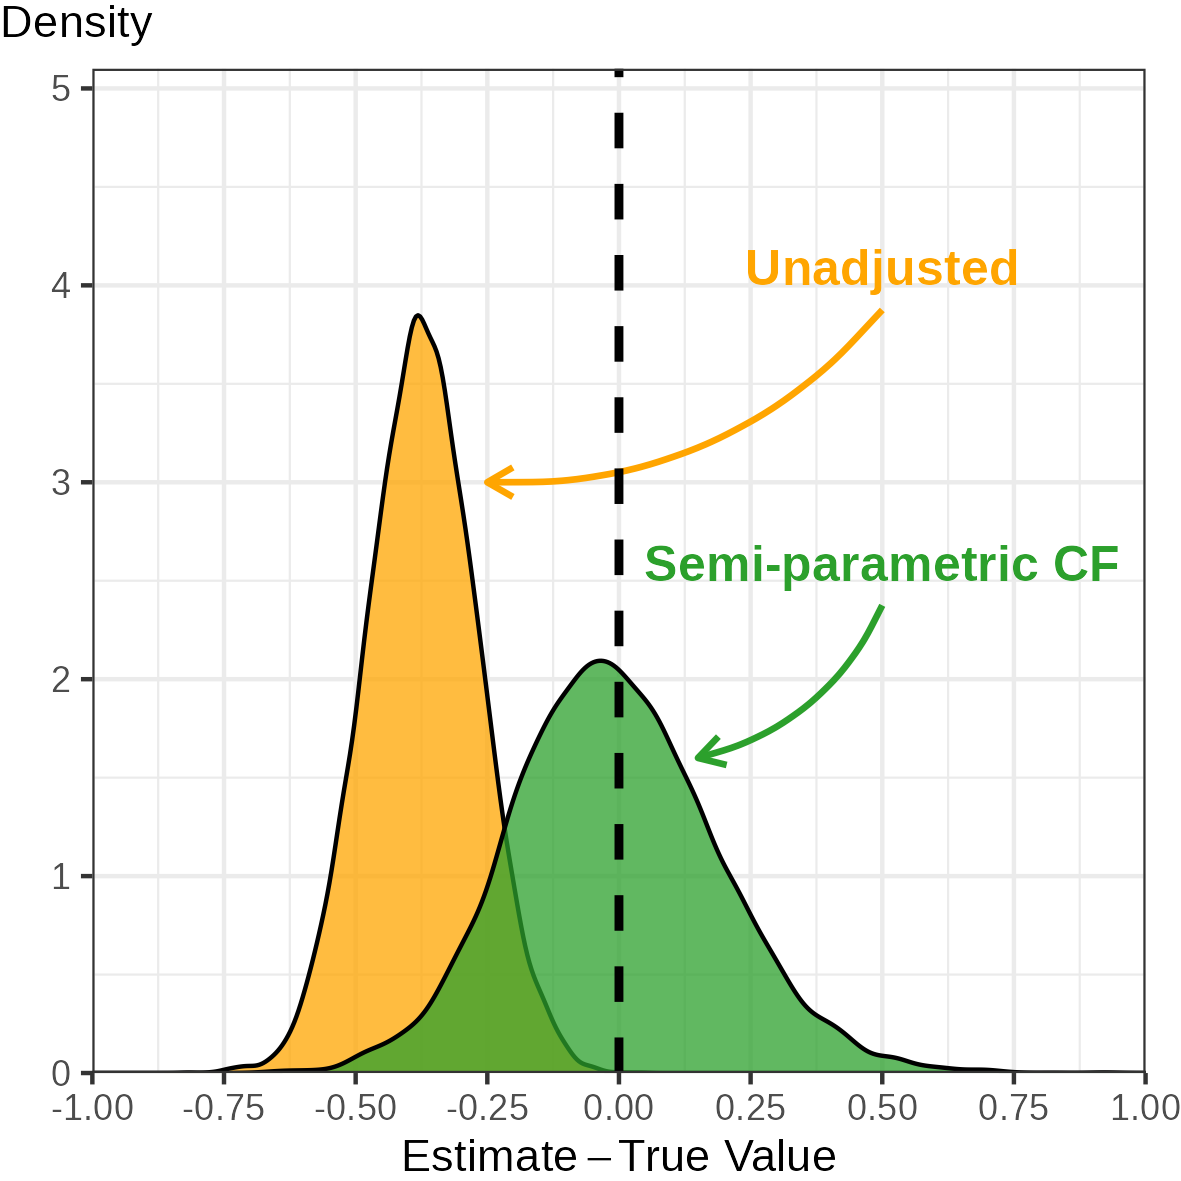
\includegraphics[width=\textwidth]{
            ../programs/simulations/sim-output/semiparametric-direct-dist.png}
    \end{subfigure}
    \begin{subfigure}[c]{0.475\textwidth}
        \centering
        \caption{$\hat{\text{AIE}} - \text{AIE}$.}
        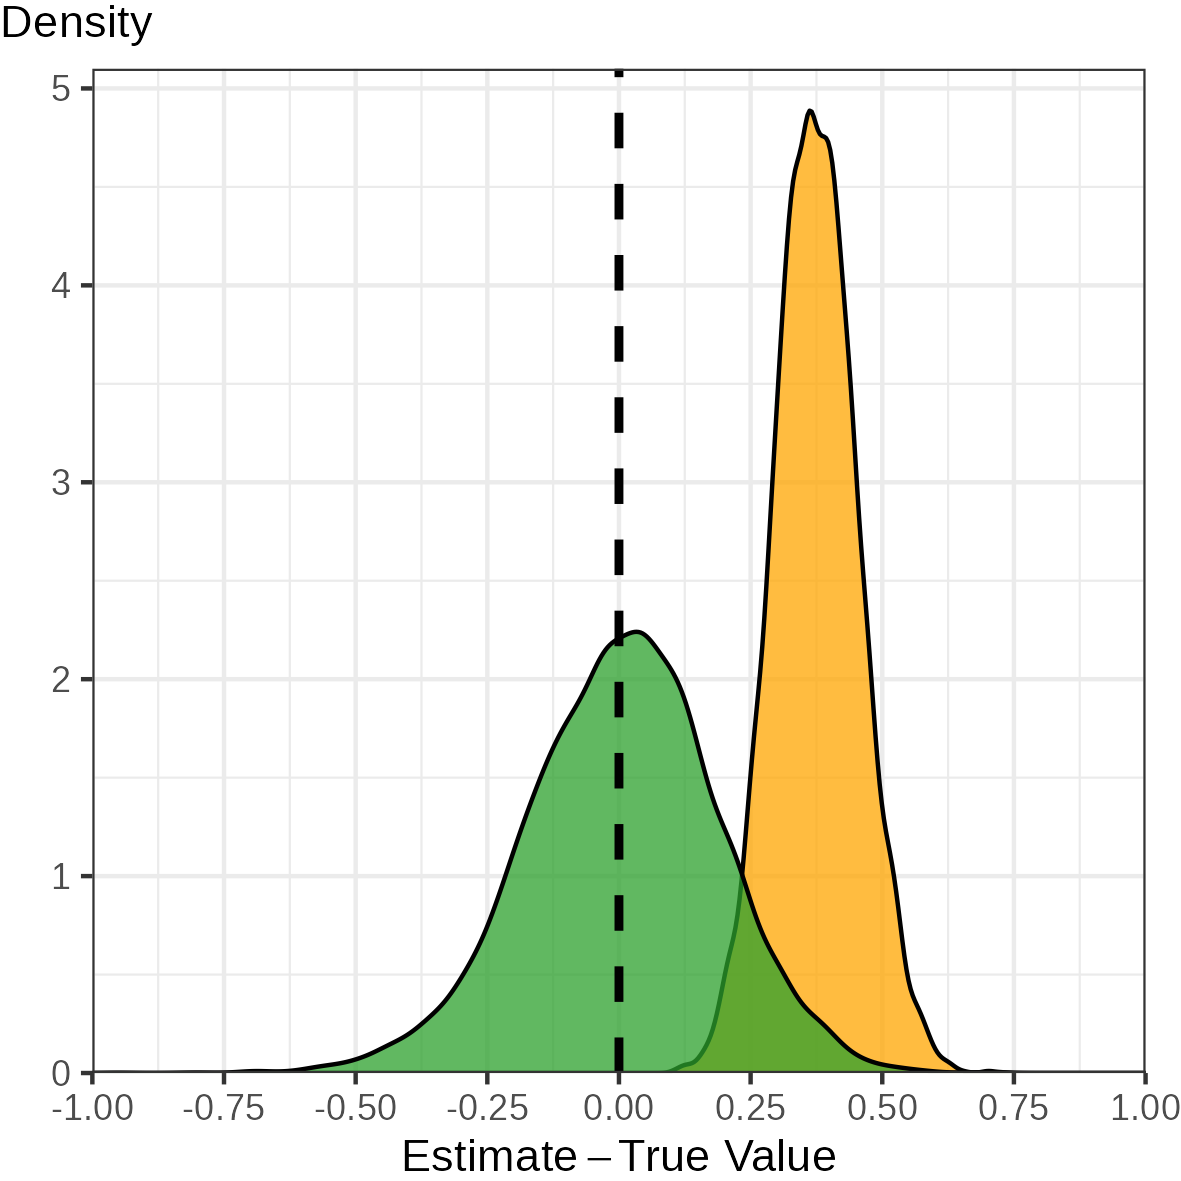
\includegraphics[width=\textwidth]{
            ../programs/simulations/sim-output/semiparametric-indirect-dist.png}
    \end{subfigure}
    \label{fig:cm-semiparametric-dist}
    \justify
    \footnotesize    
    \textbf{Note:}
    These figures show the empirical density of point estimates minus the true average effect, for 10,000 different datasets generated from a Roy model with correlated normally distributed error terms.
    The black dashed line is the true value;
    orange is the distribution of conventional CM estimates from two-stage OLS \citep{imai2010identification},
    and green estimates with a two-stage semi-parametric CF.
\end{figure}

\autoref{fig:cm-heckit-dist} shows how these estimates perform, with a parametric CF approach, relative to the true value; \autoref{fig:cm-semiparametric-dist} does the same for a semiparametric approach.
The OLS estimates' distribution do not overlap the true values for any standard level of significance; the distance between the OLS estimates and the true values are the underlying bias terms derived in \autoref{thm:selection-bias}.
The parametric CF approach perfectly reproduces the true values, as the probit first-stage correctly models the normally distributed error terms.
The semiparametric CF estimates correct conventional CM estimates, too, though exhibits some small-sample bias, which it to be expected with the involved non-parametric steps in realistic sample sizes.

\begin{figure}[h!]
    \caption{CF Adjusted Estimates Work with Different Error Term Parameters.}
    \begin{subfigure}[c]{0.475\textwidth}
        \centering
        \caption{ADE.}
        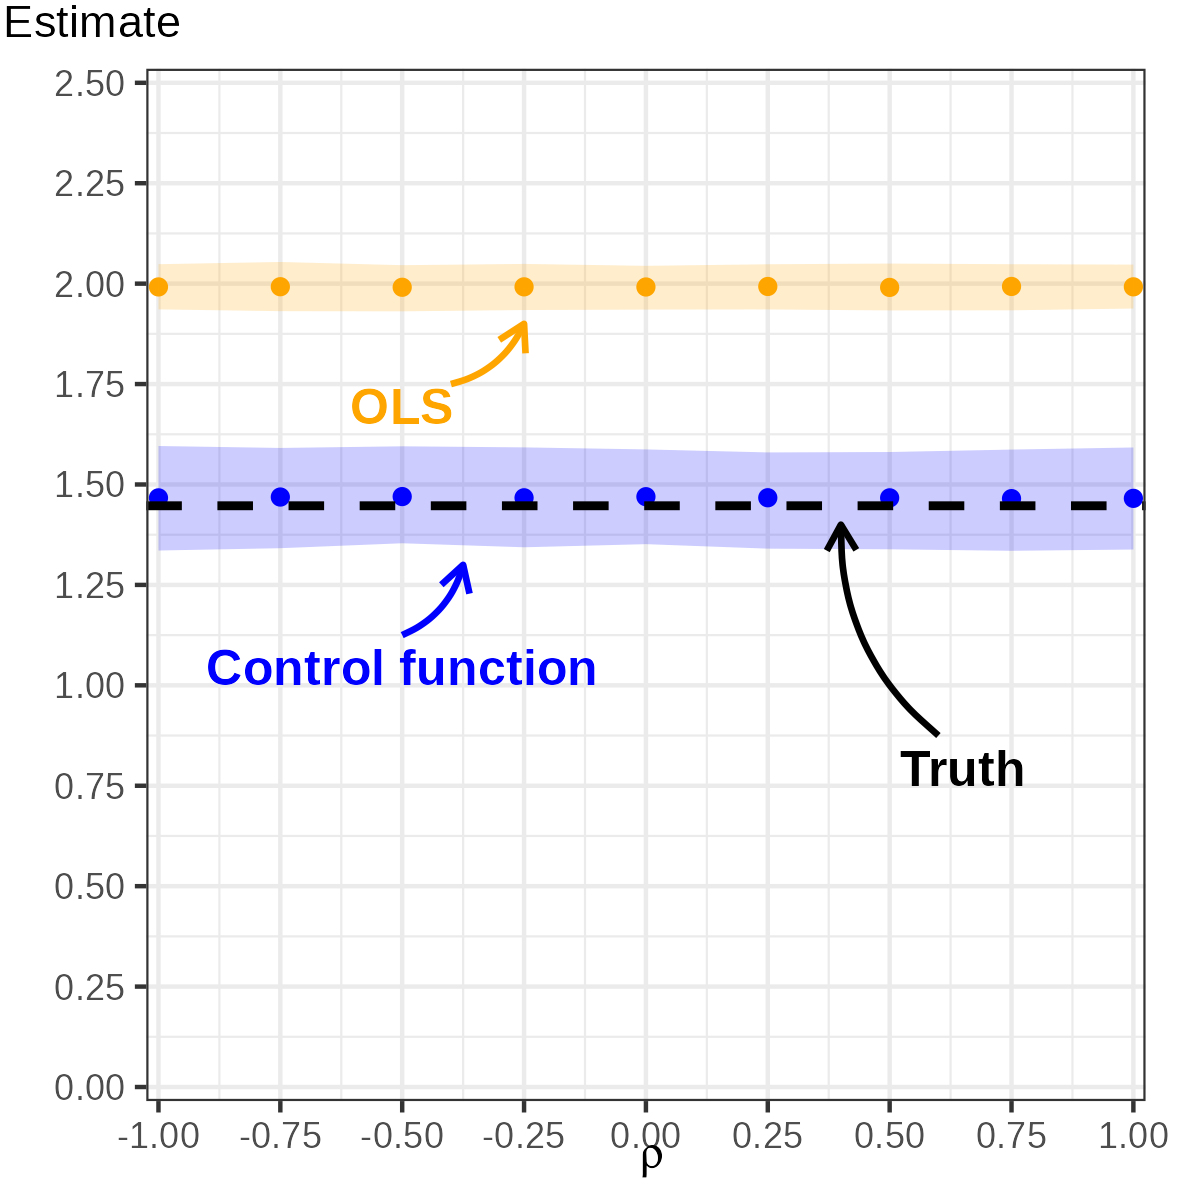
\includegraphics[width=\textwidth]{
            ../programs/simulations/sim-output/rho-directeffect-bias.png}
    \end{subfigure}
    \begin{subfigure}[c]{0.475\textwidth}
        \centering
        \caption{AIE.}
        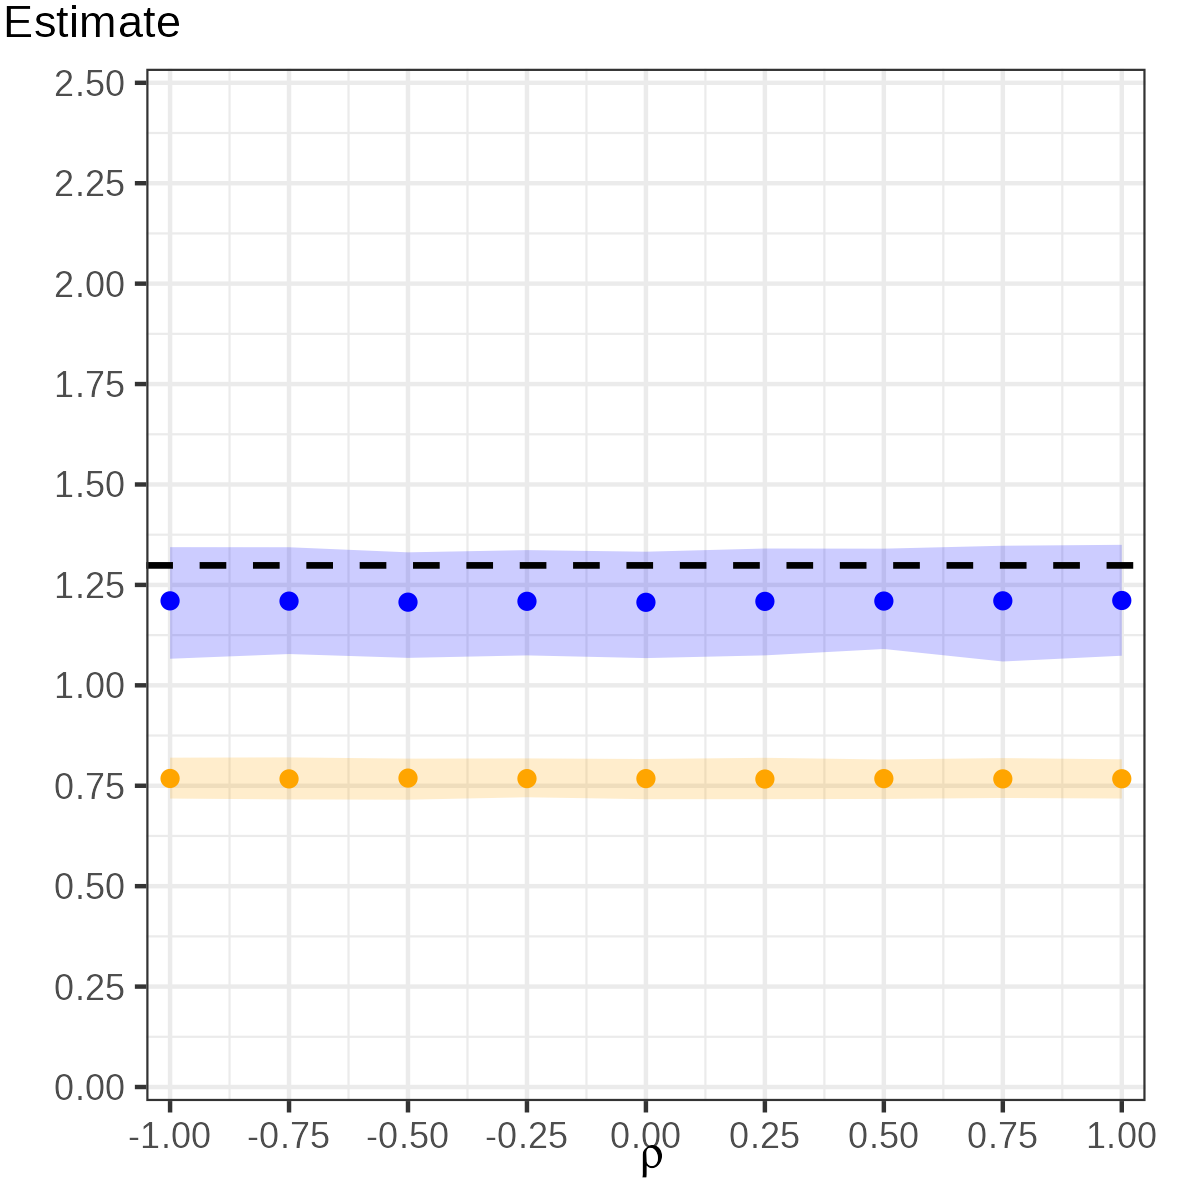
\includegraphics[width=\textwidth]{
            ../programs/simulations/sim-output/rho-indirecteffect-bias.png}
    \end{subfigure}
    \label{fig:rho-bias}
    \justify
    \footnotesize    
    \textbf{Note:}
    These figures show the OLS and CF point estimates of the ADE and AIE, for $N = 10,000$ sample size, varying $\text{Corr}\big(U_{0,i}, U_{1,i}\big)$ values with $\Var{U_{0,i}} = = 1, \Var{U_{1,i}} = 1.5$ fixed.
    The black dashed line is the true value, coloured points are points estimates for the respective data generated, and shaded regions are the 95\% confidence intervals from 1,000 bootstraps each.
    Orange represents OLS estimates, blue the CF approach.
\end{figure}

The error terms determine the bias in OLS estimates of the ADE and AIE, so the bias varies for different values of the error-term parameters $\text{Corr}\big(U_{0,i}, U_{1,i}\big) \in [-1, 1]$ and $\Var{U_{0,i}} = 1, \Var{U_{1,i}} \geq 0$.
The true AIE values vary, because $D(Z)$ compliers have higher average values of $U_{1,i} - U_{0,i}$ with greater $\text{Corr}\big(U_{0,i}, U_{1,i}\big)$ values.
\autoref{fig:rho-bias} shows CF estimates against estimates calculated by standard OLS, showing 95\% confidence intervals calculated from 1,000 bootstraps.
The point estimates of the CF do not exactly equal the true values, as they are estimates from one simulation (not averages across many simulations, as in \autoref{fig:cm-semiparametric-dist}).
The CF approach improves on OLS estimates by correcting for bias, with confidence regions overlapping the true values.\footnote{
    In the appendix, \autoref{fig:sigma-bias} shows the same simulation while varying $\Var{U_{1,i}}$, with fixed $\Var{U_{0,i}} = 1, \text{Corr}\big(U_{0,i}, U_{1,i}\big) = 0.5$.
    The conclusion is the same as for varying the correlation coefficient, $\rho$, in \autoref{fig:rho-bias}.
}
This correction did not come for free: the standard errors are significantly greater in a CF approach than OLS.
In this manner, this simulation shows the pros and cons of using the CF approach to estimating CM effects in practice.
